% 	Name		:: 	sthlm Beamer Theme  HEAVILY based on the hsrmbeamer theme (Benjamin Weiss)
%	Author		:: 	Mark Hendry Olson (mark@hendryolson.com)
%	Created		::	2013-07-31
%	Updated		::	June 18, 2015 at 08:45
%	Version		:: 	1.0.2
%	Email		:: 	hendryolson@gmail.com
%	Website		:: 	http://v42.com
%
% 	License		:: 	This file may be distributed and/or modified under the
%                  	GNU Public License.
%
%	Description	::	This presentation is a demonstration of the sthlm beamer
%					theme, which is HEAVILY based on the HSRM beamer theme created by Benjamin Weiss
%					(benjamin.weiss@student.hs-rm.de), which can be found on GitHub
%					<https://github.com/hsrmbeamertheme/hsrmbeamertheme>.


%-=-=-=-=-=-=-=-=-=-=-=-=-=-=-=-=-=-=-=-=-=-=-=-=
%
%        LOADING DOCUMENT
%
%-=-=-=-=-=-=-=-=-=-=-=-=-=-=-=-=-=-=-=-=-=-=-=-=

\documentclass[aspectratio=169, newPxFont]{beamer}
\usetheme{sthlm}
%\usecolortheme{sthlmv42}

%-=-=-=-=-=-=-=-=-=-=-=-=-=-=-=-=-=-=-=-=-=-=-=-=
%        LOADING PACKAGES
%-=-=-=-=-=-=-=-=-=-=-=-=-=-=-=-=-=-=-=-=-=-=-=-=
\usepackage[utf8]{inputenc}

\usepackage{chronology}

\renewcommand{\event}[3][e]{%
  \pgfmathsetlength\xstop{(#2-\theyearstart)*\unit}%
  \ifx #1e%
    \draw[fill=black,draw=none,opacity=0.5]%
      (\xstop, 0) circle (.2\unit)%
      node[opacity=1,rotate=45,right=.2\unit] {#3};%
  \else%
    \pgfmathsetlength\xstart{(#1-\theyearstart)*\unit}%
    \draw[fill=black,draw=none,opacity=0.5,rounded corners=.1\unit]%
      (\xstart,-.1\unit) rectangle%
      node[opacity=1,rotate=45,right=.2\unit] {#3} (\xstop,.1\unit);%
  \fi}%

%-=-=-=-=-=-=-=-=-=-=-=-=-=-=-=-=-=-=-=-=-=-=-=-=
%        BEAMER OPTIONS
%-=-=-=-=-=-=-=-=-=-=-=-=-=-=-=-=-=-=-=-=-=-=-=-=

%\setbeameroption{show notes}

%-=-=-=-=-=-=-=-=-=-=-=-=-=-=-=-=-=-=-=-=-=-=-=-=
%
%	PRESENTATION INFORMATION
%
%-=-=-=-=-=-=-=-=-=-=-=-=-=-=-=-=-=-=-=-=-=-=-=-=

%\subtitle{sthlm v1.0.0 is based on hsrm \& mTheme}
%\date{\small{\jobname}}
%\date{\today}
\author{Alysson Ribeiro, Edna Canedo}
\title{Análise de Soluções de Autenticação e Autorização para Arquiteturas Orientadas a Serviço}
\institute{Universidade de Brasília}
\setbeamercovered{transparent} 
\setbeamertemplate{footline}[frame number]

\begin{document}

%-=-=-=-=-=-=-=-=-=-=-=-=-=-=-=-=-=-=-=-=-=-=-=-=
%
%	TITLE PAGE
%
%-=-=-=-=-=-=-=-=-=-=-=-=-=-=-=-=-=-=-=-=-=-=-=-=



\begin{frame}[plain]
	\titlepage
\end{frame}

\begin{frame}
	\tableofcontents
\end{frame}

\section{Introdução}
		\begin{frame}{Barramento Orientado a Serviço - ESB }
		\begin{figure}[h!]
		\begin{center}
		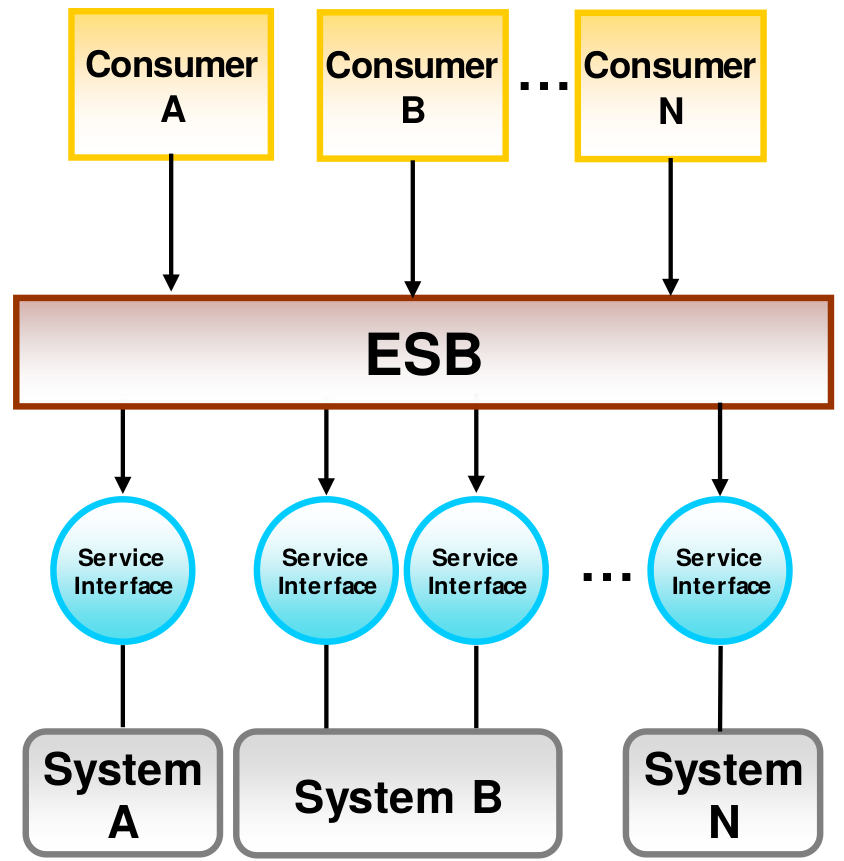
\includegraphics[scale = 0.22]{img/ESB.png}
		\label{fun:fig:oauth}
		\end{center}
	\end{figure} 


		\end{frame}

		\begin{frame}{Barramento Orientado a Serviço - ESB }
			\begin{itemize}
				\item Apoiar a modernização dos sistemas legados da UnB;
				\item Oferece integração entre as aplicações;
				\item Evita duplicidade de código;
			\end{itemize}
		\end{frame}

	\begin{frame}{Problema}
		\begin{itemize}
			\item Encontrar um padrão seguro para integração através do ESB;
			\begin{itemize}
				\item Confidencialidade
				\item Autenticidade
				\item Integralidade
				\item Disponibilidade
			\end{itemize}
		\end{itemize}
	\end{frame}
	
\begin{frame}{Objetivo}
		\fontsize{20}{\baselineskip} \selectfont{
Realizar um mapeamento sistemático para identificar os principais desafios e soluções sobre autenticação e autorização em SOA.}
\end{frame}

\section{Mapeamento Sistemático}

\begin{frame}{Questões de Pesquisa}
	\begin{description}

		\item[QP1)] Quais os principais protocolos utilizados para autenticação e autorização em SOA?
		\item[QP2)] Quais os principais estilos arquiteturais abordados nos estudos?% Quantos estudos abordam a utilização de um ESB?
	\end{description}
\end{frame}

\begin{frame}{\textit{String} de Busca}
		\fontsize{17}{\baselineskip} \selectfont{
	\textbf{\textit{((Authentication AND authorization) OR "Access Control" OR Security) AND (SOA OR ESB OR REST)}}}
\end{frame}

\begin{frame}{Critérios de Inclusão}
	\begin{description}
		\item [CI1)]Período compreendido do ano de 2006 até 2016. 
		\item [CI2)] Gratuitos nos idiomas inglês ou português. 
	\end{description}
	
\end{frame}

\begin{frame}{Critérios de Exclusão}
	\begin{description}
		\item [CE1)]Não tratam de autenticação ou autorização em SOA;
		\item [CE2)]Estudos incompletos;
		\item [CE3)]Estudos com menos de quatro páginas.
	\end{description}
\end{frame}



\begin{frame}{Processo de Extração dos Dados}
	\begin{table}[htbp]
		\centering
		\begin{tabular}{r|c|c|ccc|c}
			\toprule
			\textbf{}&\multicolumn{2}{c}{\textbf{Etapa 1}} & \multicolumn{4}{c}{\textbf{Etapa 2}} \\
			\midrule
			\textbf{Fontes} & \textbf{Estudos} & \textbf{Estudos} & \multicolumn{3}{c}{\textbf{Excluídos}} & \textbf{Incluídos} \\
			\textbf{} & \textbf{retornados} & \textbf{Relevantes} & \textbf{QE1} & \textbf{QE2} & \textbf{QE3} & \textbf{} \\
			\textbf{IEEE} & 45    & 38    & 11     & 2     & 3     & \multicolumn{1}{c}{\textbf{22}} \\
			\textbf{ACM} & 89    & 24    & 8     & 0     & 0     & \multicolumn{1}{c}{\textbf{16}} \\
			\textbf{ScienceDirect} & 2238  & 10    & 5     & 0     & 0     & \multicolumn{1}{c}{\textbf{5}} \\
			\textbf{Springer Link} & 1893  & 10     & 7     & 0     & 2     & \multicolumn{1}{c}{\textbf{2}} \\ 
			\midrule
			\textbf{Total} & 4265  & 82    & 31    & 2     & 5     & \multicolumn{1}{c}{\textbf{44}} \\
			\bottomrule
		\end{tabular}%
		\label{tab:addlabel}%
	\end{table}%	
\end{frame}


\begin{frame}{Processo de Extração dos Dados}
			\begin{center}
				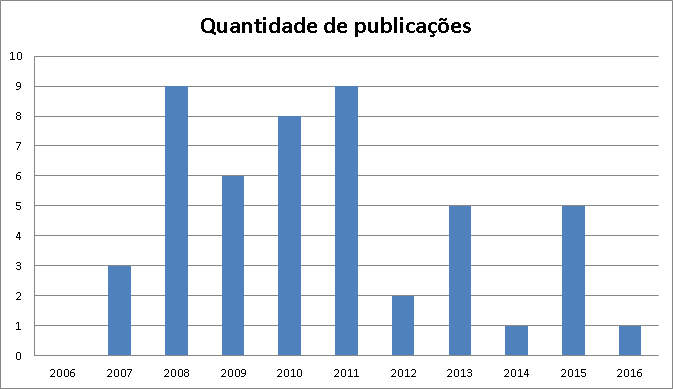
\includegraphics[scale = 0.65]{img/ano.png}
			\end{center}
\end{frame}


\section{Resultados}
\begin{frame}{Questão de Pesquisa 1}
	\begin{center}
		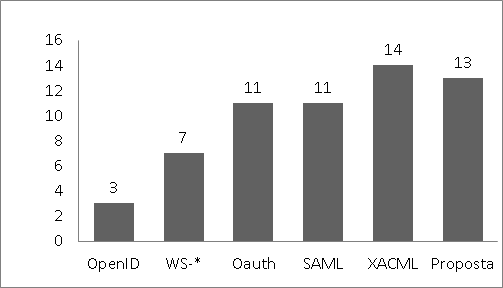
\includegraphics[scale = 0.8]{img/protocolos.png}
	\end{center}
\end{frame}

\begin{frame}{Questão de Pesquisa 2}
	\begin{center}
		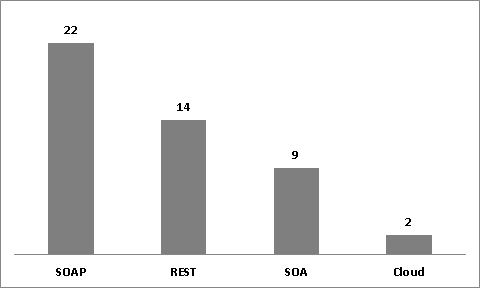
\includegraphics[scale = 0.8]{img/estilo.png}
	\end{center}
\end{frame}

%\begin{frame}{Questão de Pesquisa 3}
%		\fontsize{25}{\baselineskip} \selectfont{\textbf{Performance}} 
%\end{frame}

\section{Conclusões}
\begin{frame}{Conclusão}
	Esse estudo possibilitou:
	\begin{itemize}
		\item Selecionar 44 estudos relacionados com o tema;
		\item Identificar as principais soluções em Autenticação e Autorização em SOA;
	\end{itemize}
\end{frame}

\begin{frame}{Trabalhos Futuros}
	\begin{enumerate}
		\item Identificar quais os problemas de autenticação e autorização em SOA e quais as soluções utilizadas para REST;
		\item Selecionar ou propor um protocolo adequado para a UnB;
		\item Implementar o protocolo;
		\item Realizar estudos de caso para testar e validar o protocolo.
	\end{enumerate}
\end{frame}

\begin{frame}{FIM}
	\fontsize{30}{\baselineskip} \selectfont{\textbf{Obrigado!}}
\end{frame}
\end{document}